\documentclass[12pt]{article}

\usepackage{sbc-template}
\usepackage{graphicx,url}
\usepackage[brazil]{babel}   
\usepackage[utf8]{inputenc}  
\usepackage[T1]{fontenc}

\usepackage{microtype}
\usepackage[caption=false]{subfig}
\usepackage{bm}
\usepackage{amsmath,amsfonts,amssymb}
\usepackage{booktabs,longtable}

\usepackage{algpseudocode}
\usepackage[linesnumbered,ruled,vlined]{algorithm2e}
\SetArgSty{textnormal}
\DontPrintSemicolon

\sloppy

\title{Metaheurística GRASP com refinamento por busca local para o Flowshop Permutacional}

\author{Alberto F. K. Neto\inst{1}}

\address{Instituto de Informática -- Universidade Federal do Rio Grande do Sul
  (UFRGS)\\
  Caixa Postal 15.064 -- 91.501-970 -- Porto Alegre -- RS -- Brazil
  \email{afkneto@inf.ufrgs.br} 
}

\begin{document} 

\maketitle

\section{Introdução}

Este relatório refere-se ao trabalho de otimização da disciplina de Otimização
Combinatória (INF05010), cursada no período de 2019/1. O texto apresenta o
problema de otimização considerado e introduz um modelo de Programação Linear
Inteira da literatura do problema. Detalhes sobre o desenvolvimento de um método
de solução heurístico baseado em GRASP e Busca Local encontram-se disponíveis
nas seções indicadas, e o desempenho do método proposto é comparado com os
melhores valores de solução atualmente conhecidos para um pequeno conjunto de
instâncias de teste. 

\section{Descrição do problema}

O Problema de Flowshop Permutacional (PFSP) é um tema de pesquisa recorrente
nos estudos da otimização combinatória. O problema considera um conjunto de 
$M$ máquinas e $N$ tarefas, em que todas as tarefas devem ser processadas 
exatamente uma vez em cada uma das máquinas consideradas. Cada tarefa 
$1 \leqslant j \leqslant N$ demora $T_{rj} \geqslant 0$ unidades de tempo para ser 
processada cada máquina $1 \leqslant r \leqslant M$. Busca-se uma ordem de
execução das tarefas que minimize o tempo final de processamento da última 
máquina considerada. Essa ordem de execução é seguida por todas as máquinas.

\cite{tseng2004-flowshop-models} propuseram um modelo de programação linear
inteira mista para o problema. As variáveis binárias $D_{ik} \in \{0,1\}$
assumem o valor $1$ para indicar
se a tarefa $i$ deve ser processada em algum momento anterior ao 
processamento da tarefa $k$, com $1 \leqslant i < k \leqslant N$.
Já as variáveis contínuas $C_{ri} \geqslant 0$ indicam o horizonte de tempo 
de processamento que cada tarefa $ 1 \leqslant i \leqslant N$ em cada
máquina $1 \leqslant r \leqslant M$.
Adicionamente, a variável $C_\mathrm{max} \geqslant 0$ é utilizado no
cálculo do tempo final de processamento da última máquina. 
De posse dessas definições, a seguinte formulação modela o Problema de 
Flowshop permutacional. Note a existência de um parâmetro $P$, que é um 
número suficientemente grande usado como ``big-M'' na modelagem das 
restrições lógicas do modelo.

\clearpage 

\begin{align}
   \text{Minimize } C_\mathrm{max} \label{pfsp:obj}
\end{align}
Sujeito a:
\begin{align}
   & C_{1i} \geqslant T_{1i} & & 1 \leqslant i \leqslant N \label{pfsp:complM0} \\
   & C_{ri} - C_{r-1,i} \geqslant T_{ri} & & 2 \leqslant r \leqslant M, 
      1 \leqslant i \leqslant N \label{pfsp:complM} \\
   & C_{ri} - C_{rk} + PD_{ik} \geqslant T_{ri} & & 1 \leqslant r \leqslant M, 
      1 \leqslant i < k \leqslant N \label{pfsp:jobSeqA}\\
   & C_{ri} - C_{rk} + PD_{ik} \leqslant P - T_{rk} & & 1 \leqslant r \leqslant M, 
      1 \leqslant i < k \leqslant N \label{pfsp:jobSeqB} \\
   & C_\mathrm{max} \geqslant C_{Mi} & & 1 \leqslant i \leqslant N \label{pfsp:makespan} \\
   & C_{ri} \geqslant 0 & & 1 \leqslant r \leqslant M, 1 \leqslant i \leqslant N \label{pfsp:Cdom}\\
   & D_{ik} \in \{0,1\} & & 1 \leqslant i < k \leqslant N \label{pfsp:Ddom}
\end{align}

A função objetivo (\ref{pfsp:obj}) minimiza o tempo de processamento final da
última máquina do problema. As restrições (\ref{pfsp:complM0}) e
(\ref{pfsp:complM}) modelam o tempo final de processamento das tarefas na
primera e demais máquinas, respectivamente. As restrições
(\ref{pfsp:jobSeqA}--\ref{pfsp:jobSeqB}) garantem uma única ordem de execução 
das tarefas em todas as máquinas. A restrição (\ref{pfsp:makespan}) calcula o
tempo final de processamento da última máquina. Por fim, as restrições
(\ref{pfsp:Cdom}--\ref{pfsp:Ddom}) modelam o domínio das variáveis de decisão do
problema.

\section{Método de solução com GRASP e Busca Local}

Tendo em vista a questão da típica baixa eficiência de métodos exatos em
resolver problemas de otimização combinatória discreta, propõe-se o seguinte
método de solução heurístico para resolução do problema. O método de solução é
implementa umaa heurística GRASP para construção de uma soluçãoa inicial
\cite{feo1994-grasp}, seguida de uma fase de intensificação com busca local. 
O pseudocódigo dos algoritmos de construção inicial e de busca local são 
listados em \ref{algo:GRASP} e \ref{algo:LS}. 
Na notação a seguir, uma solução é definida como uma lista com a ordem de
processamento das tarefas, e pode ser parcial ou completa.
Uma visão geral do método de
solução está disponível no algoritmo \ref{algo:full}.

\begin{algorithm}[H]
   \footnotesize
   \SetKwFunction{proc}{GRASP}
   \SetKwProg{myproc}{Procedure}{}{}
   \myproc{\proc{$N$, $M$, $T$, $\alpha$}}{
      $\mathit{pend} \gets$ lista com valores $1, 2, \dots, N$ \;
      $s \gets $ lista vazia; $z \gets 0$ \;
      \While{$\mathit{pend}$ não está vazia}{
         $\mathit{RCL} \gets $ lista vazia \;
         \For{$j \in \mathit{pend}$}{
            $\bar{z}_j \gets$ custo da solução parcial $s$ com adição da tarefa $j$ \; 
            adicione a tupla $(j, \bar{z}_j)$ em $\mathit{RCL}$ \;
         }
         ordene $\mathit{RCL}$ em ordem não crescente de $\bar{z}$ \;
         $\mathit{tam} \gets$ tamanho da lista $\mathit{RCL}$ \;
         $\mathit{tp} \gets$ escolhe aleatoriamente um índice 
            de $[1, \max\{1, \alpha \cdot \mathit{tam}\} ]$ \;
         atualize a solução $s$ e custo $z$ com os dados da tupla $\mathit{RCL}_\mathit{tp}$ \;
         remova a tarefa referente a $\mathit{tp}$ de $\mathit{pend}$ \;
      }
   }
   \Return{$s$}
   \caption{Construção de solução inicial com GRASP.}
   \label{algo:GRASP}
\end{algorithm}

O algoritmo GRASP inicial com uma solução vazia, de custo 0, e incrementalmente
adiciona tarefas na ordem de processamento das máquinas. Inicialmente, todas as
tarefas são marcadas como pendentes (lista $\mathit{pend}$). A cada iteração do 
laço principal
(linhas 4--13), calcula-se o custo de inserção de cada tarefa pendente
na solução parcial $s$. Esses valores de custo são adicionados à
lista $\mathit{RCL}$ de tarefas candidatas a entrar na solução. Faz-se a
ordenação dessa lista em ordem não crescente de custo de solução,
e escolhe-se aleatoriamente uma das $\alpha$\% tarefas iniciais da lista de
candidatos. Essa tarefa entra na solução parcial $s$, e o custo $z$ é
atualizado de acordo. Finalmente, a tarefa é removida da lista de pendentes e
a próxima iteração inicia. Essa implementação de GRASP faz a seleção com
$\alpha$ pelos índices da lista de candidatos.

\begin{algorithm}[H]
   \footnotesize
   \SetKwFunction{proc}{Swap2LS}
   \SetKwProg{myproc}{Procedure}{}{}
   \myproc{\proc{$s^*$, numVezes}}{
      $z^* \gets$ custo da solução atual\;
      \For {$i \gets 1$ até $numVezes$} {
         selecione tarefas $j_1 \neq j_2$ aleatoriamente, com distribuição uniforme \;
         $\bar{s} \gets$ troque a ordem de processamento de $j_1 \leftrightarrow j_2$ em $s^*$ \;
         $\bar{z} \gets$ avalie o custo da solução $\bar{s}$ \;
         \If {$\bar{z} < z^*$} {
            $s^* \gets \bar{s}$ \;
            $z^* \gets \bar{z}$ \;
         }
      }
   }
   \Return $s*$
   \caption{Algoritmo de Busca Local iterada com trocas aleatória.}
   \label{algo:LS}
\end{algorithm}

Após a construção de uma solução inicial com GRASP, inicia-se a fase de
melhoramento da solução com o algoritmo de busca local iterado \ref{algo:LS}.
A busca local faz diversas tentativas de troca da ordem de processamento de
duas tarefas em posições distintas, e sempre aceita a troca na ordem das
tarefas caso seja vantajosa (estratégia de ``primeira melhora''). De posse de
ambos os algoritmos, é possível definir o método de solução completo como em
\ref{algo:full}.

\begin{algorithm}[H]
   \footnotesize
   \SetKwFunction{proc}{GRASP\_LS}
   \SetKwProg{myproc}{Procedure}{}{}
   \myproc{\proc{$N$, $M$, $T$, $\alpha$}}{
      $s \gets$ \texttt{GRASP}($N$, $M$, $T$, $\alpha$) \;
      \For{$\mathit{iter} \gets 1$ até $\textit{MAX\_ITER}$ } {
         \texttt{Swap2LS}($s$, $\lceil N/100 \rceil$) \;
         \texttt{Swap2LS}($s$, $\lceil \mathit{iter}/1000 \rceil$) \;
         \texttt{Swap2LS}($s$, \texttt{randomInt}(1,N)) \;
      }
   }
   \Return $s$
   \caption{Algoritmo completo da heurística GRASP com Busca Local.}
   \label{algo:full}
\end{algorithm}

Como consideração final, todas as seleções aleatórias se deram
por distribuição uniforme. Utilizou-se cada uma das replicações 
$n=1, \dots, 10$ da heurística como semente do gerador de números
pseudoaleatórios.

\section{Resultados computacionais}

Os testes computacionais da heurística e da formulação matemática foram
conduzidos nas instâncias de teste indicadas na definição do trabalho da
disciplinas. Utilizou-se um computador Intel 3612QM @ 2.10GHz, dispondo-se de
8 GB de memória principal. A heurística foi implementada em Python 
3.7.4, e o modelo foi resolvido por meio do GLPK 4.65. O ambiente de testes foi
o Arch Linux de 64 bits, com kernel padrão 5.3.8.


\begin{table}[ht]
   \begin{tabular}{lrrrr}
      \toprule
      Instância & BKS & Valor relaxação & Obj. solução inteira & GAP$_\mathrm{BKS}$ (\%) \\
      \midrule
      VFR10\_15\_1 & 1307 & 880.0 & 1307 & \phantom{0}0.0\\
      VFR10\_10\_3 & 1592 & 687.0 & 1873 & 56.9\\
      VFR\_20\_20\_1 & 2270 & 1391.0 & 2573 & 42.6\\
      VFR60\_5\_10 & 3663 & 382.0 & 3878 & 89.3\\
      VFR100\_60\_1 & 9395  &  TL & -- & $\infty$\\
      VFR500\_40\_1 & 28548 &  TL & -- & $\infty$\\
      VFR500\_60\_3 & 31125 &  TL & -- & $\infty$\\
      VFR600\_20\_1 & 31433 &  TL & -- & $\infty$\\
      VFR700\_20\_10 & 36417 & TL & -- & $\infty$\\ 
      \bottomrule
   \end{tabular}
\end{table}

\section{Conclusões}

% \begin{figure}
%    \centering
%    \subfloat[][]{
%       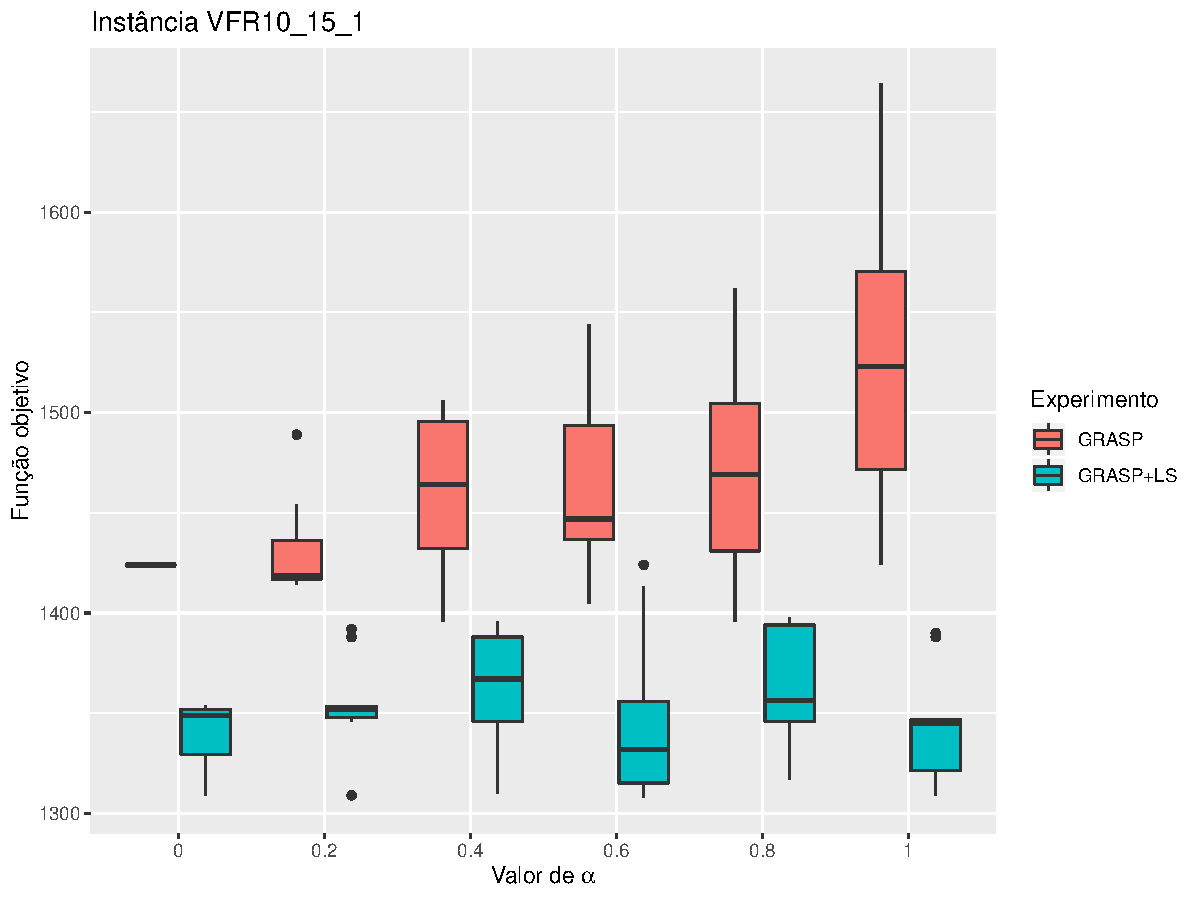
\includegraphics[width=0.48\textwidth]{../resultados/boxplot-VFR10_15_1.pdf}
%    }
%    \subfloat[][]{
%       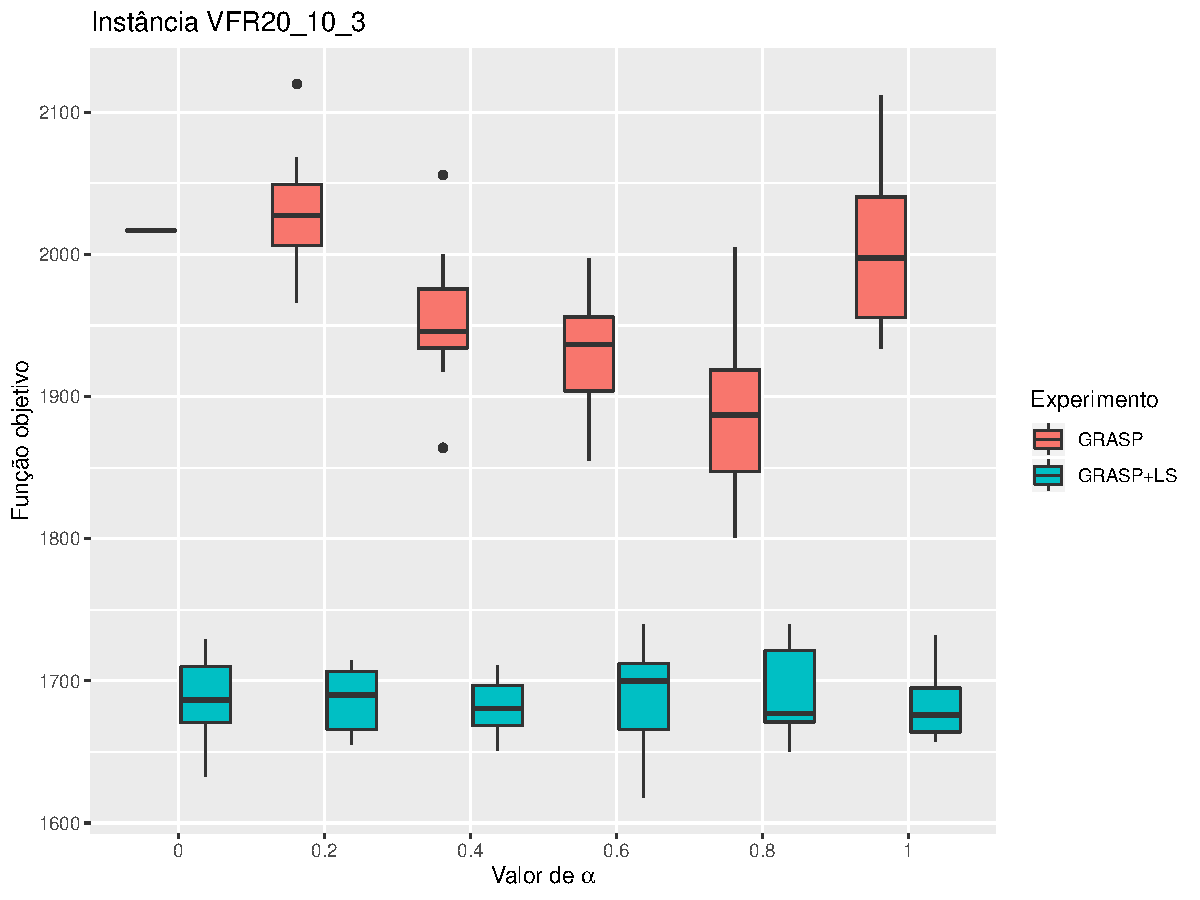
\includegraphics[width=0.48\textwidth]{../resultados/boxplot-VFR20_10_3.pdf}
%    }\\
%    \subfloat[][]{
%       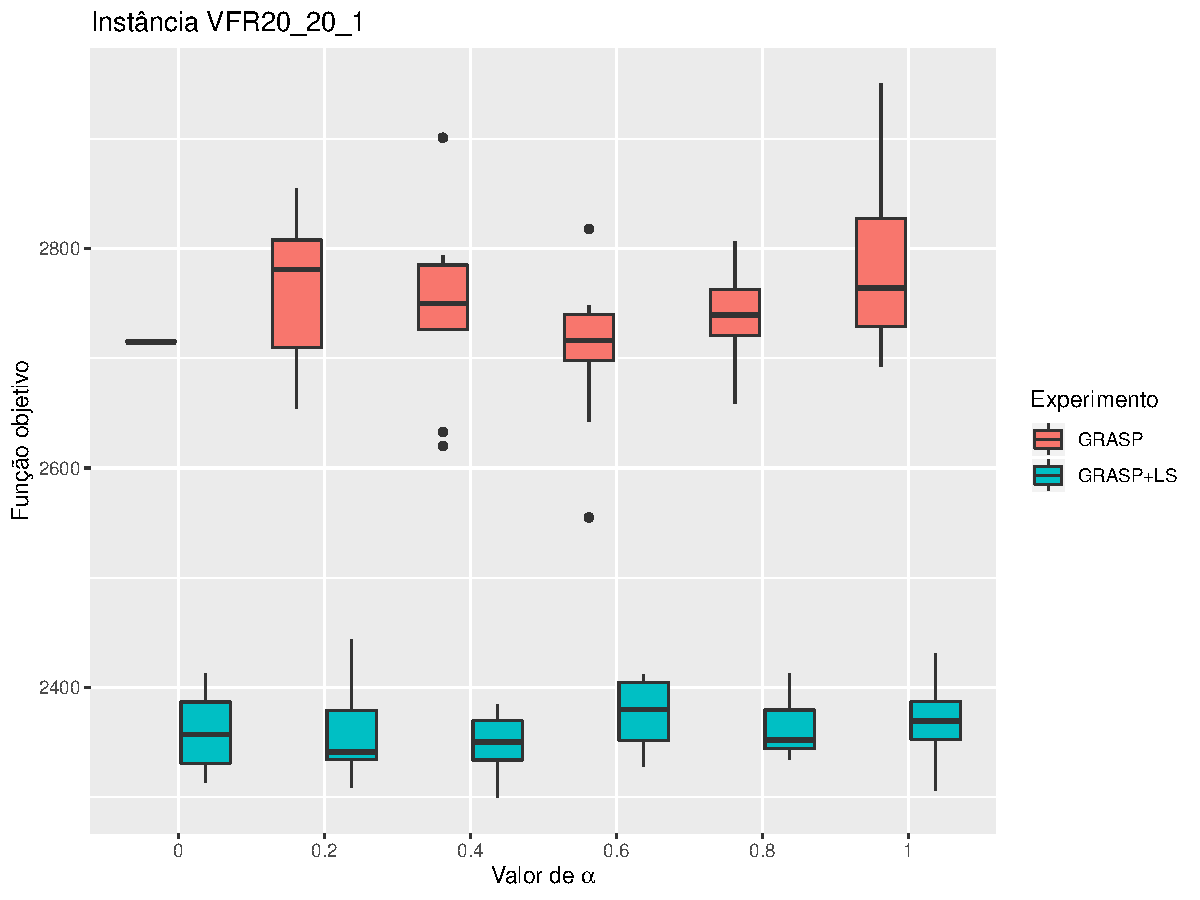
\includegraphics[width=0.48\textwidth]{../resultados/boxplot-VFR20_20_1.pdf}
%    }
%    \subfloat[][]{
%       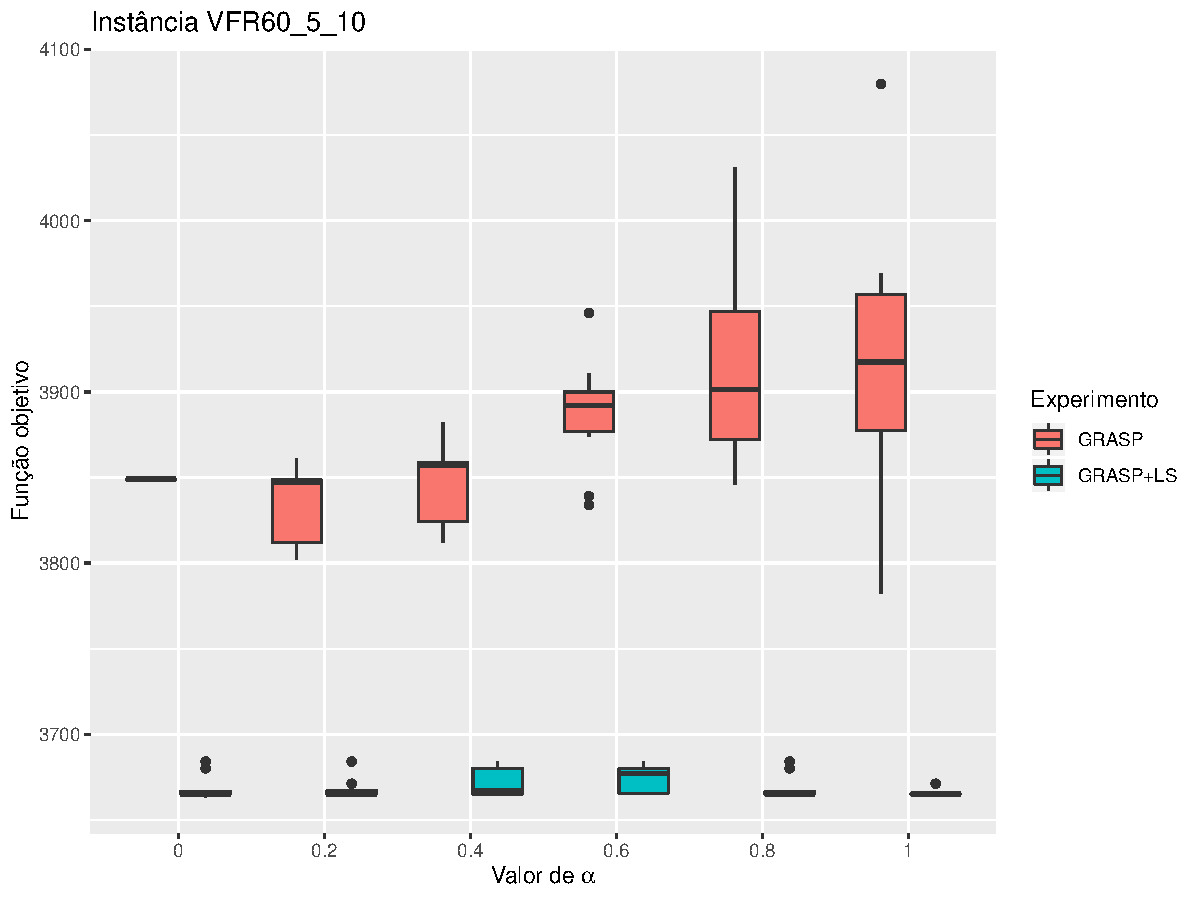
\includegraphics[width=0.48\textwidth]{../resultados/boxplot-VFR60_5_10.pdf}
%    }\\
%    \subfloat[][]{
%       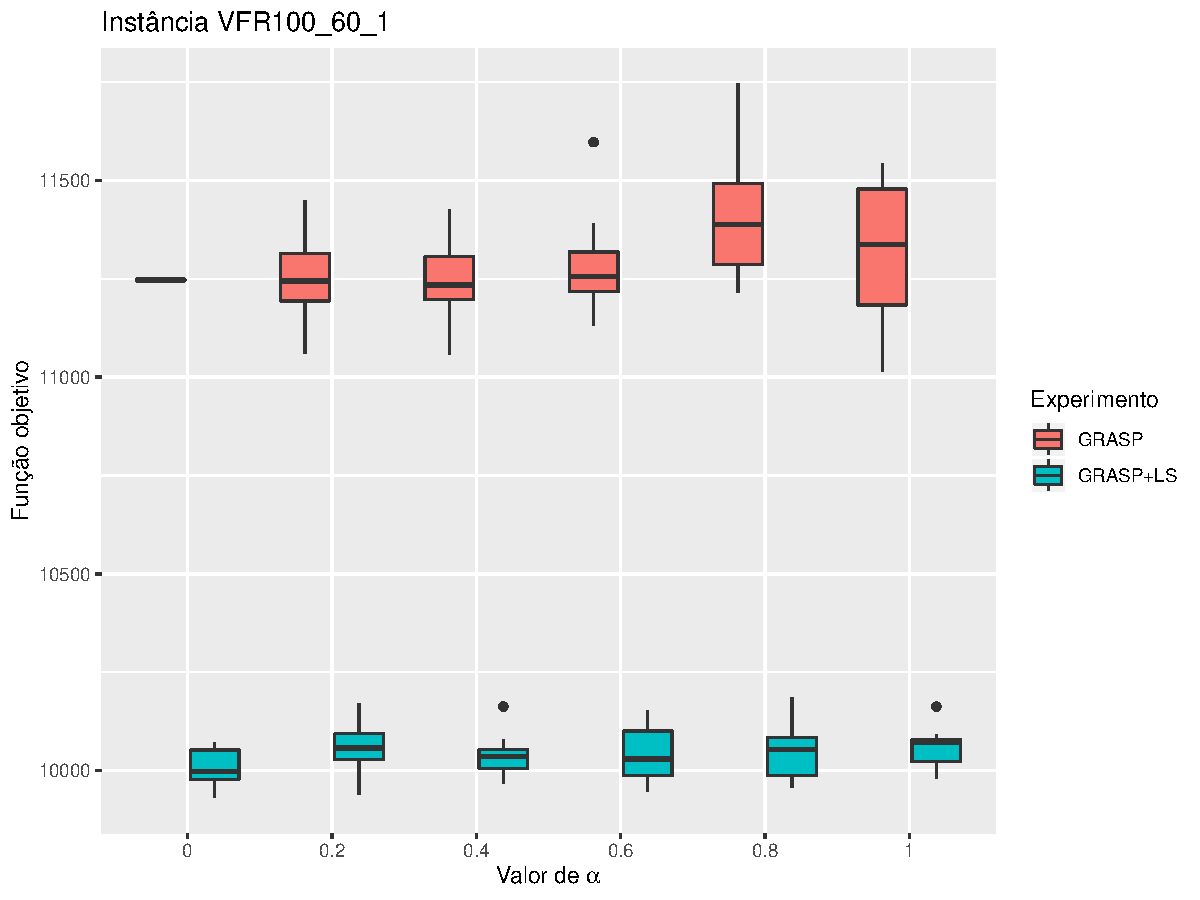
\includegraphics[width=0.48\textwidth]{../resultados/boxplot-VFR100_60_1.pdf}
%    }
%    \subfloat[][]{
%       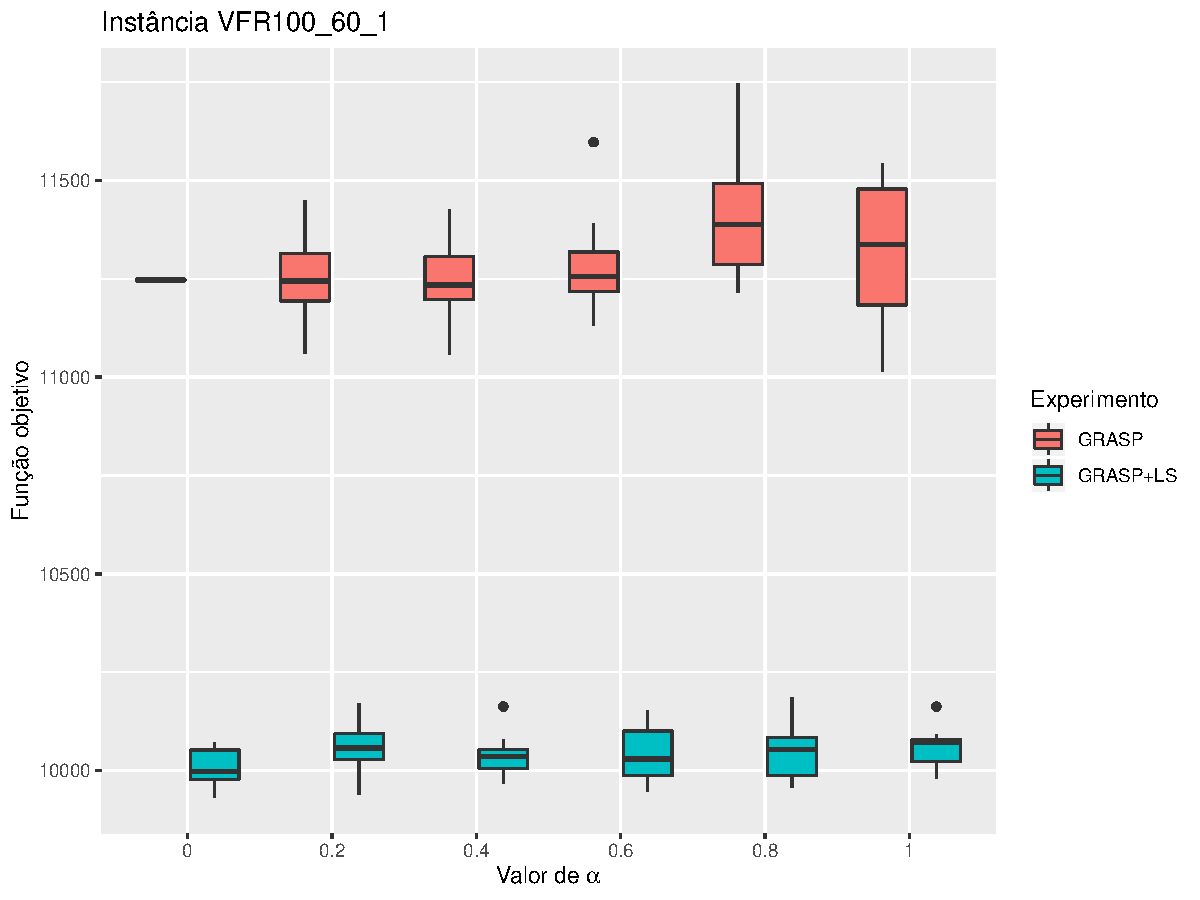
\includegraphics[width=0.48\textwidth]{../resultados/boxplot-VFR100_60_1.pdf}
%    }
%    \caption{Boxplot relacionando valor médio da função objetivo para as diversas 
%       instâncias de testes, com vários valores \bm{$\alpha$} e 10 replicações
%       por caso de teste.}
% \end{figure}
% 
% \begin{figure}
%    \ContinuedFloat
%    \subfloat[][]{
%       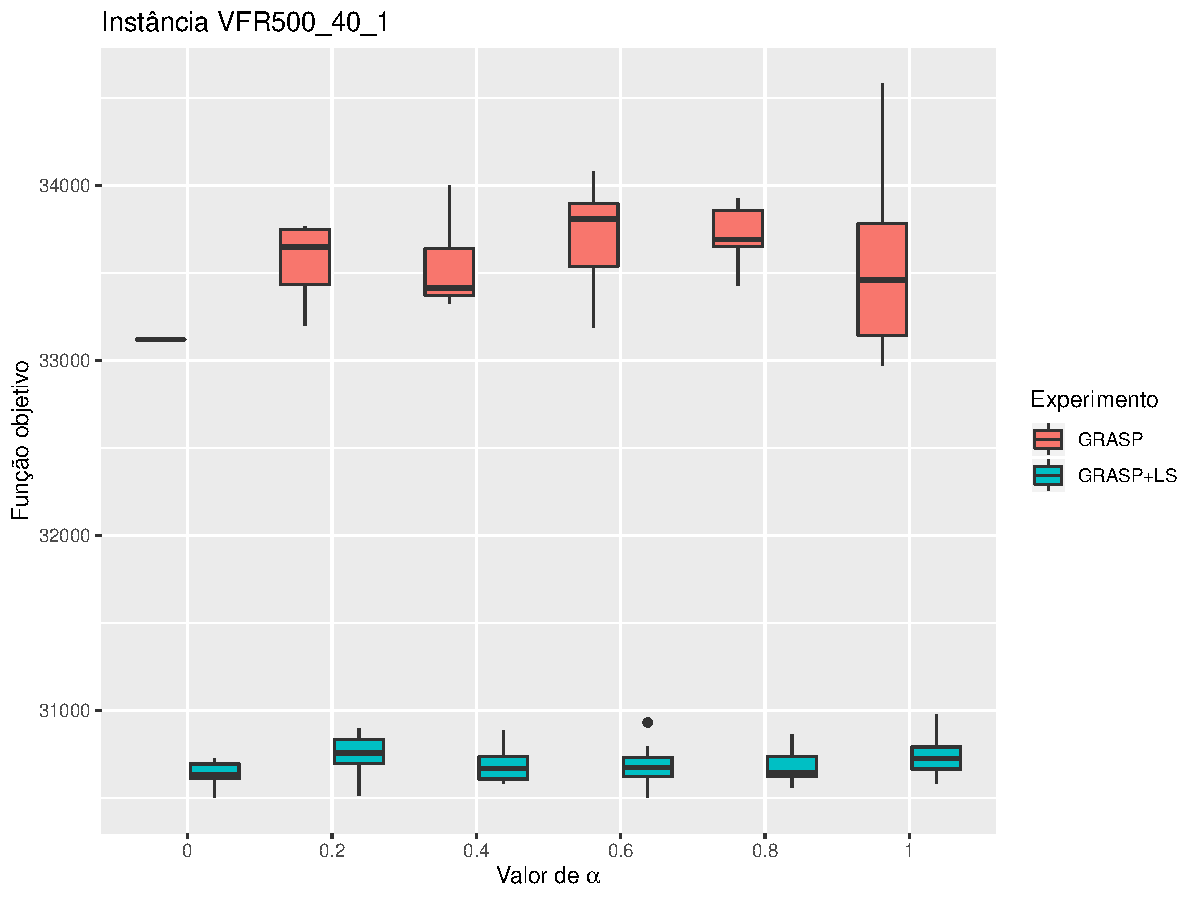
\includegraphics[width=0.48\textwidth]{../resultados/boxplot-VFR500_40_1.pdf}
%    }
%    \subfloat[][]{
%       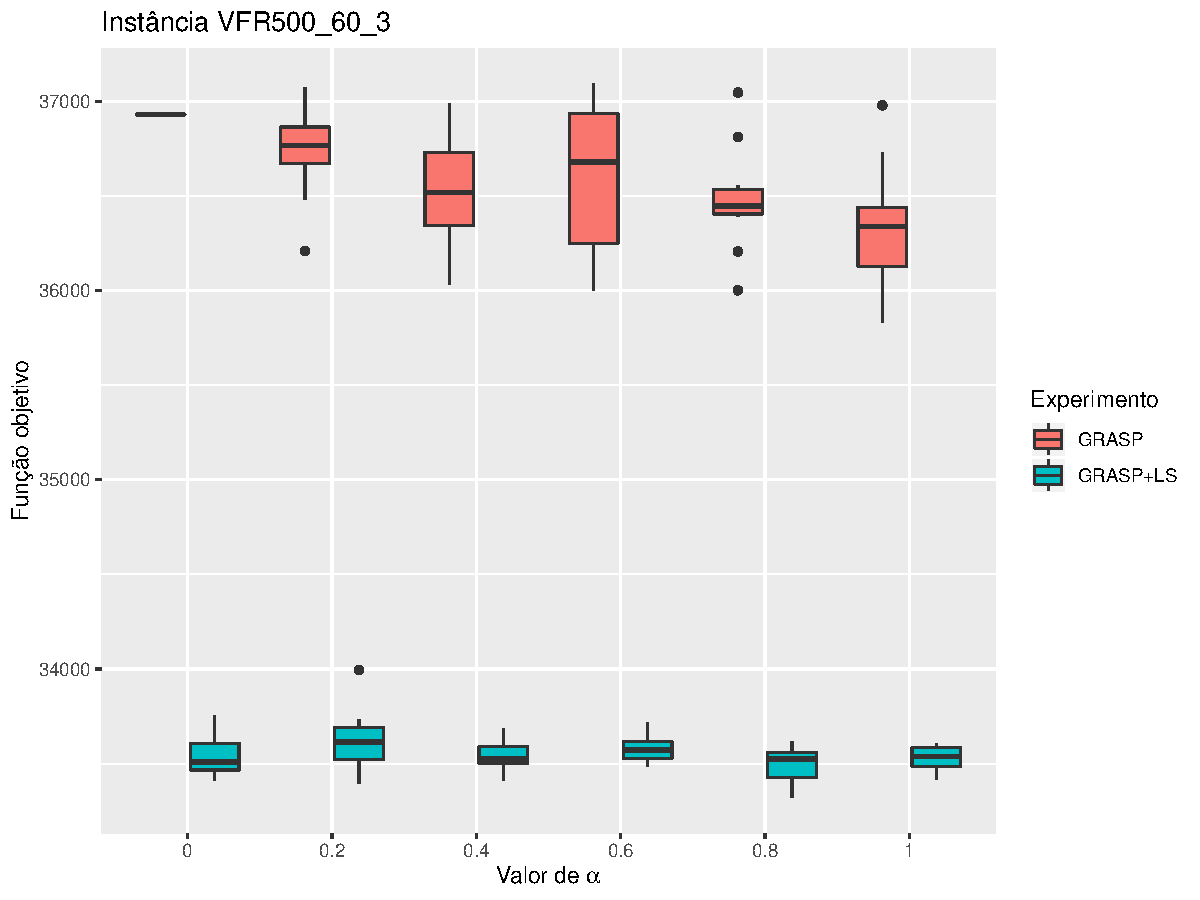
\includegraphics[width=0.48\textwidth]{../resultados/boxplot-VFR500_60_3.pdf}
%    }\\
%    \subfloat[][]{
%       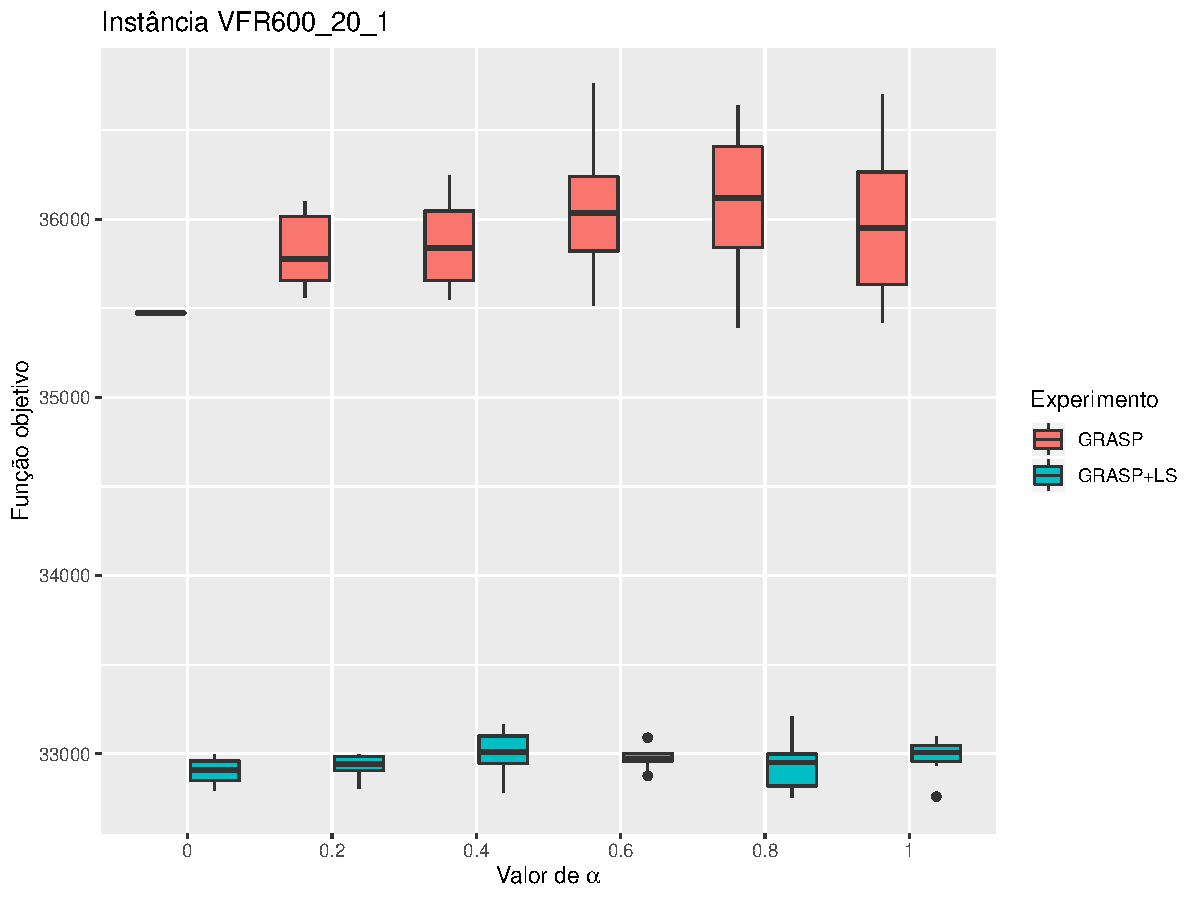
\includegraphics[width=0.48\textwidth]{../resultados/boxplot-VFR600_20_1.pdf}
%    }
%    \subfloat[][]{
%       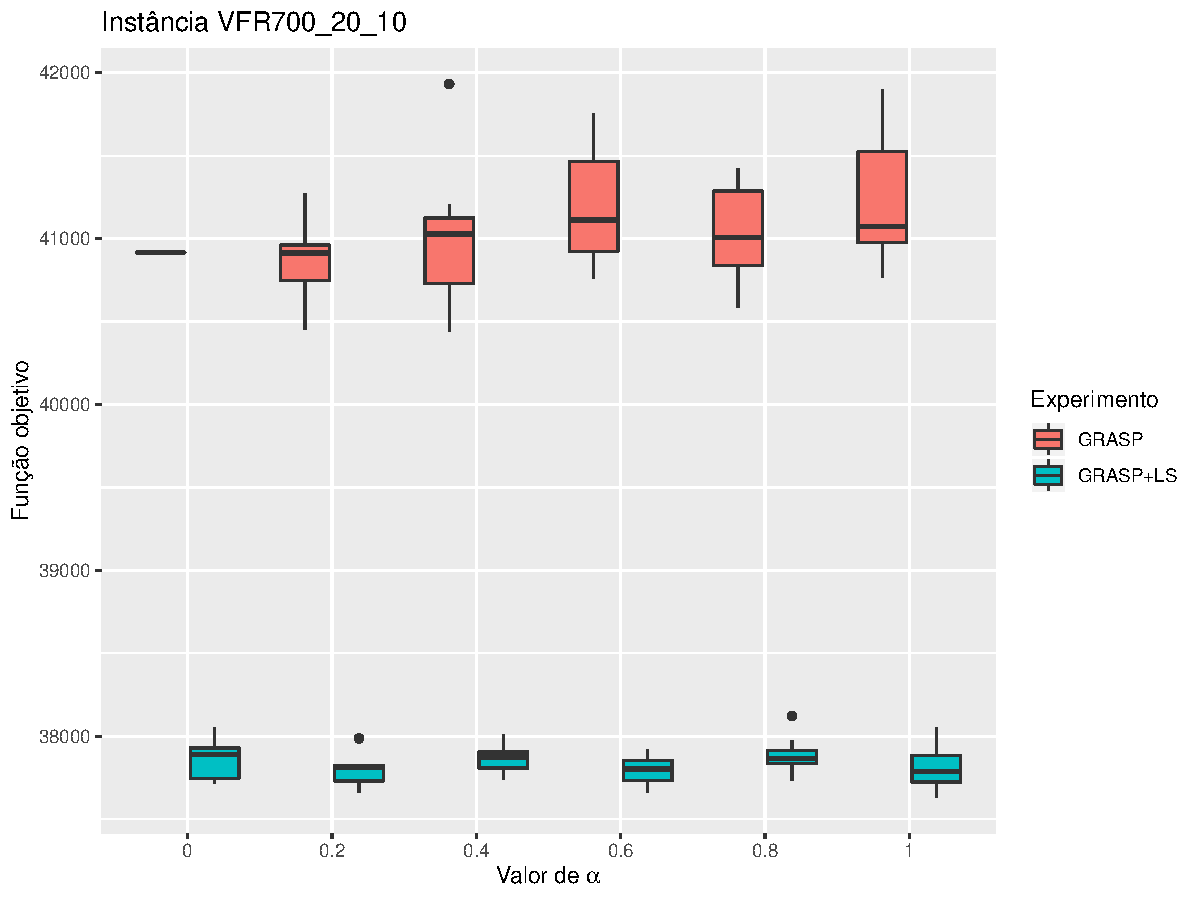
\includegraphics[width=0.48\textwidth]{../resultados/boxplot-VFR700_20_10.pdf}
%    }
%    \caption{Boxplot relacionando valor médio da função objetivo para as diversas 
%       instâncias de testes, com vários valores \bm{$\alpha$} e 10 replicações
%       por caso de teste. Continuação da figura anterior.}
% \end{figure}

\bibliographystyle{sbc}
\bibliography{referencias}

\appendix

\section*{Apêndice A -- Média dos resultados computacionais para diversos
\protect{$\alpha$}}

\tiny
% latex table generated in R 3.6.1 by xtable 1.8-4 package
% Fri Nov  1 11:27:33 2019
\begin{longtable}{lrrccccr}
\toprule
\multirow{2}{*}{Instância} & \multirow{2}{*}{BKS} & \multicolumn{3}{c}{Sol.
GRASP} & \multicolumn{3}{c}{Sol. GRASP + Busca Local}\\ \cmidrule(r){3-5}
\cmidrule(l){6-8}
& & $\alpha$ & Valor F.O. & GAP$_\mathrm{BKS}$ (\%) & Valor F.O &
GAP$_\mathrm{BKS}$ (\%) & Tempo (seg.) \\ 
\midrule
\endhead

\bottomrule
\endfoot


 VFR10\_15\_1 & 1307.00 & 0.00 & $1424 \pm 0$ & 8.95 & $1339.6 \pm 18.319$ & 2.49 & $1.5 \pm 0.04$ \\ 
  VFR10\_15\_1 & 1307.00 & 0.20 & $1431.5 \pm 24.024$ & 9.53 & $1354.2 \pm 23.011$ & 3.61 & $1.4 \pm 0.03$ \\ 
  VFR10\_15\_1 & 1307.00 & 0.40 & $1459.6 \pm 39.884$ & 11.68 & $1364.2 \pm 28.944$ & 4.38 & $1.5 \pm 0.04$ \\ 
  VFR10\_15\_1 & 1307.00 & 0.60 & $1465.8 \pm 43.827$ & 12.15 & $1346.1 \pm 42.331$ & 2.99 & $1.4 \pm 0.03$ \\ 
  VFR10\_15\_1 & 1307.00 & 0.80 & $1470.6 \pm 49.934$ & 12.52 & $1362.9 \pm 30.205$ & 4.28 & $1.5 \pm 0.04$ \\ 
  VFR10\_15\_1 & 1307.00 & 1.00 & $1528.7 \pm 75.588$ & 16.96 & $1342.2 \pm 28.867$ & 2.69 & $1.5 \pm 0.03$ \\ 
   \midrule
VFR100\_60\_1 & 9395.00 & 0.00 & $11247 \pm 0$ & 19.71 & $10008.8 \pm 47.123$ & 6.53 & $57.7 \pm 0.59$ \\ 
  VFR100\_60\_1 & 9395.00 & 0.20 & $11251.8 \pm 118.302$ & 19.76 & $10054.5 \pm 70.099$ & 7.02 & $57.7 \pm 0.42$ \\ 
  VFR100\_60\_1 & 9395.00 & 0.40 & $11243.3 \pm 121.401$ & 19.67 & $10039.1 \pm 54.017$ & 6.86 & $57.9 \pm 0.52$ \\ 
  VFR100\_60\_1 & 9395.00 & 0.60 & $11287.2 \pm 131.908$ & 20.14 & $10040.9 \pm 73.843$ & 6.87 & $58.5 \pm 0.87$ \\ 
  VFR100\_60\_1 & 9395.00 & 0.80 & $11409.9 \pm 164.966$ & 21.45 & $10048.8 \pm 69.904$ & 6.96 & $58 \pm 1$ \\ 
  VFR100\_60\_1 & 9395.00 & 1.00 & $11312.1 \pm 187.334$ & 20.41 & $10057.8 \pm 55.519$ & 7.05 & $58.2 \pm 0.99$ \\ 
   \midrule
VFR20\_10\_3 & 1592.00 & 0.00 & $2017 \pm 0$ & 26.70 & $1687.5 \pm 29.304$ & 6.00 & $2.1 \pm 0.05$ \\ 
  VFR20\_10\_3 & 1592.00 & 0.20 & $2030.4 \pm 44.443$ & 27.54 & $1685.8 \pm 23.223$ & 5.89 & $2 \pm 0.03$ \\ 
  VFR20\_10\_3 & 1592.00 & 0.40 & $1954.6 \pm 51.036$ & 22.78 & $1682 \pm 21.417$ & 5.65 & $2 \pm 0.03$ \\ 
  VFR20\_10\_3 & 1592.00 & 0.60 & $1931 \pm 47.044$ & 21.29 & $1690.8 \pm 39.6$ & 6.21 & $2 \pm 0.04$ \\ 
  VFR20\_10\_3 & 1592.00 & 0.80 & $1894.9 \pm 65.665$ & 19.03 & $1692.3 \pm 32.094$ & 6.30 & $2 \pm 0.02$ \\ 
  VFR20\_10\_3 & 1592.00 & 1.00 & $2007.5 \pm 64.24$ & 26.10 & $1682.7 \pm 24.157$ & 5.70 & $2 \pm 0.04$ \\ 
   \midrule
VFR20\_20\_1 & 2270.00 & 0.00 & $2715 \pm 0$ & 19.60 & $2360.1 \pm 33.478$ & 3.97 & $3.9 \pm 0.07$ \\ 
  VFR20\_20\_1 & 2270.00 & 0.20 & $2759.4 \pm 69.617$ & 21.56 & $2355.8 \pm 41.214$ & 3.78 & $3.9 \pm 0.08$ \\ 
  VFR20\_20\_1 & 2270.00 & 0.40 & $2745.8 \pm 80.5$ & 20.96 & $2350 \pm 25.573$ & 3.52 & $3.9 \pm 0.08$ \\ 
  VFR20\_20\_1 & 2270.00 & 0.60 & $2706.7 \pm 69.72$ & 19.24 & $2376.6 \pm 31.178$ & 4.70 & $3.9 \pm 0.06$ \\ 
  VFR20\_20\_1 & 2270.00 & 0.80 & $2735.3 \pm 44.475$ & 20.50 & $2362.9 \pm 26.236$ & 4.09 & $3.8 \pm 0.05$ \\ 
  VFR20\_20\_1 & 2270.00 & 1.00 & $2787.7 \pm 84.592$ & 22.81 & $2366.9 \pm 38.766$ & 4.27 & $3.9 \pm 0.07$ \\ 
   \midrule
VFR500\_40\_1 & 28548.00 & 0.00 & $33119 \pm 0$ & 16.01 & $30640.6 \pm 67.832$ & 7.33 & $200.4 \pm 8.47$ \\ 
  VFR500\_40\_1 & 28548.00 & 0.20 & $33572.6 \pm 207.304$ & 17.60 & $30753.7 \pm 111.634$ & 7.73 & $200 \pm 4.51$ \\ 
  VFR500\_40\_1 & 28548.00 & 0.40 & $33516.3 \pm 217.696$ & 17.40 & $30697.4 \pm 107.934$ & 7.53 & $197.2 \pm 1.52$ \\ 
  VFR500\_40\_1 & 28548.00 & 0.60 & $33720.7 \pm 278.457$ & 18.12 & $30681.7 \pm 127.513$ & 7.47 & $198.4 \pm 1.59$ \\ 
  VFR500\_40\_1 & 28548.00 & 0.80 & $33710.1 \pm 176.109$ & 18.08 & $30688.4 \pm 101.606$ & 7.50 & $199.6 \pm 3.45$ \\ 
  VFR500\_40\_1 & 28548.00 & 1.00 & $33522.1 \pm 494.424$ & 17.42 & $30741.5 \pm 113.56$ & 7.68 & $200.9 \pm 7.53$ \\ 
   \midrule
VFR500\_60\_3 & 31125.00 & 0.00 & $36930 \pm 0$ & 18.65 & $33539.6 \pm 106.966$ & 7.76 & $298.5 \pm 4.31$ \\ 
  VFR500\_60\_3 & 31125.00 & 0.20 & $36741.8 \pm 257.954$ & 18.05 & $33624.6 \pm 167.947$ & 8.03 & $300.7 \pm 3.79$ \\ 
  VFR500\_60\_3 & 31125.00 & 0.40 & $36508.5 \pm 314.718$ & 17.30 & $33535.1 \pm 81.036$ & 7.74 & $299.2 \pm 3.89$ \\ 
  VFR500\_60\_3 & 31125.00 & 0.60 & $36596.7 \pm 410.012$ & 17.58 & $33576.6 \pm 71.104$ & 7.88 & $300.6 \pm 3.38$ \\ 
  VFR500\_60\_3 & 31125.00 & 0.80 & $36482.3 \pm 288.909$ & 17.21 & $33490.7 \pm 96.158$ & 7.60 & $298.3 \pm 3.3$ \\ 
  VFR500\_60\_3 & 31125.00 & 1.00 & $36327 \pm 354.164$ & 16.71 & $33530.5 \pm 65.58$ & 7.73 & $298.7 \pm 2.61$ \\ 
   \midrule
VFR60\_10\_3 & 3423.00 & 0.00 & $4357 \pm 0$ & 27.29 & $3632.6 \pm 62.45$ & 6.12 & $6 \pm 0.06$ \\ 
  VFR60\_10\_3 & 3423.00 & 0.20 & $4367.2 \pm 83.639$ & 27.58 & $3637.4 \pm 67.612$ & 6.26 & $6 \pm 0.14$ \\ 
  VFR60\_10\_3 & 3423.00 & 0.40 & $4334.5 \pm 93.77$ & 26.63 & $3630.7 \pm 55.041$ & 6.07 & $6 \pm 0.08$ \\ 
  VFR60\_10\_3 & 3423.00 & 0.60 & $4305 \pm 84.374$ & 25.77 & $3608.3 \pm 50.557$ & 5.41 & $5.9 \pm 0.11$ \\ 
  VFR60\_10\_3 & 3423.00 & 0.80 & $4430.9 \pm 112.114$ & 29.44 & $3603.6 \pm 72.537$ & 5.28 & $6 \pm 0.08$ \\ 
  VFR60\_10\_3 & 3423.00 & 1.00 & $4390.9 \pm 136.315$ & 28.28 & $3626.3 \pm 54.214$ & 5.94 & $6 \pm 0.09$ \\ 
   \midrule
VFR60\_5\_10 & 3663.00 & 0.00 & $3849 \pm 0$ & 5.08 & $3668.4 \pm 7.291$ & 0.15 & $3.2 \pm 0.09$ \\ 
  VFR60\_5\_10 & 3663.00 & 0.20 & $3833.2 \pm 22.25$ & 4.65 & $3667.9 \pm 5.971$ & 0.13 & $3.2 \pm 0.13$ \\ 
  VFR60\_5\_10 & 3663.00 & 0.40 & $3847.5 \pm 24.699$ & 5.04 & $3672.2 \pm 8.574$ & 0.25 & $3.1 \pm 0.05$ \\ 
  VFR60\_5\_10 & 3663.00 & 0.60 & $3887.3 \pm 33.002$ & 6.12 & $3674.4 \pm 8.03$ & 0.31 & $3.2 \pm 0.06$ \\ 
  VFR60\_5\_10 & 3663.00 & 0.80 & $3917.5 \pm 60.99$ & 6.95 & $3668.6 \pm 7.152$ & 0.15 & $3.2 \pm 0.03$ \\ 
  VFR60\_5\_10 & 3663.00 & 1.00 & $3914 \pm 87.271$ & 6.85 & $3665.6 \pm 1.897$ & 0.07 & $3.1 \pm 0.05$ \\ 
   \midrule
VFR600\_20\_1 & 31433.00 & 0.00 & $35473 \pm 0$ & 12.85 & $32904.4 \pm 69.306$ & 4.68 & $118.4 \pm 1.86$ \\ 
  VFR600\_20\_1 & 31433.00 & 0.20 & $35828.1 \pm 208.495$ & 13.98 & $32930 \pm 65.09$ & 4.76 & $121.1 \pm 5.56$ \\ 
  VFR600\_20\_1 & 31433.00 & 0.40 & $35865.6 \pm 235.46$ & 14.10 & $32999.7 \pm 123.094$ & 4.98 & $119.3 \pm 1.99$ \\ 
  VFR600\_20\_1 & 31433.00 & 0.60 & $36042.2 \pm 370.703$ & 14.66 & $32982.4 \pm 68.39$ & 4.93 & $119.2 \pm 1.82$ \\ 
  VFR600\_20\_1 & 31433.00 & 0.80 & $36070.7 \pm 419.604$ & 14.75 & $32932.5 \pm 134.142$ & 4.77 & $123.1 \pm 9.14$ \\ 
  VFR600\_20\_1 & 31433.00 & 1.00 & $35964.1 \pm 425.271$ & 14.42 & $32990.1 \pm 97.588$ & 4.95 & $122.6 \pm 7.68$ \\ 
   \midrule
VFR700\_20\_10 & 36417.00 & 0.00 & $40916 \pm 0$ & 12.35 & $37857.4 \pm 114.996$ & 3.96 & $140.6 \pm 2.03$ \\ 
  VFR700\_20\_10 & 36417.00 & 0.20 & $40858.5 \pm 222.473$ & 12.20 & $37792.3 \pm 93.295$ & 3.78 & $140 \pm 3.16$ \\ 
  VFR700\_20\_10 & 36417.00 & 0.40 & $41003.3 \pm 407.564$ & 12.59 & $37865.9 \pm 79.689$ & 3.98 & $139 \pm 2.11$ \\ 
  VFR700\_20\_10 & 36417.00 & 0.60 & $41196.8 \pm 355.395$ & 13.13 & $37798.9 \pm 87.46$ & 3.79 & $142.6 \pm 9.19$ \\ 
  VFR700\_20\_10 & 36417.00 & 0.80 & $41036.6 \pm 281.03$ & 12.69 & $37882.2 \pm 110.235$ & 4.02 & $140.3 \pm 3.43$ \\ 
  VFR700\_20\_10 & 36417.00 & 1.00 & $41214.5 \pm 385.111$ & 13.17 & $37807.6 \pm 124.189$ & 3.82 & $139.8 \pm 2.51$ \\ 




 
\end{longtable}

\normalsize

\end{document}
